\documentclass[submit]{harvardml}

% FDV: Check all frontmatter for years, due dates, and references for
% sections of the textbook, etc.
\course{CS181-S22}
\assignment{Assignment \#3}
\duedate{11:59pm EST, March 11, 2022}

\usepackage[OT1]{fontenc}
\usepackage[colorlinks,citecolor=blue,urlcolor=blue]{hyperref}
\usepackage[pdftex]{graphicx}
\usepackage{subfig}
\usepackage{fullpage}
\usepackage{amsmath}
\usepackage{amssymb}
\usepackage{color}
\usepackage{soul}
\usepackage{todonotes}
\usepackage{listings}
\usepackage{common}
\usepackage{enumitem}
\usepackage{bm}
\usepackage{physics}
\newcommand{\B}{\text{B}}
\newcommand{\Beta}{\text{Beta}}
\usepackage{pythonhighlight}
\usepackage[mmddyyyy,hhmmss]{datetime}
\newcommand{\wmean}{\vb{w}_{\text{mean}}}
\newcommand{\what}{\hat{\vb{w}}}
\newcommand{\E}{\mathbb{E}}


\setlength\parindent{0em}

\definecolor{verbgray}{gray}{0.9}

\lstnewenvironment{csv}{%
  \lstset{backgroundcolor=\color{verbgray},
  frame=single,
  framerule=0pt,
  basicstyle=\ttfamily,
  columns=fullflexible}}{}

\begin{document}

\begin{center}
{\Large Homework 3: Bayesian Methods and Neural Networks}\\
\end{center}

% FDV: Update for resources, accuracy of submit information **especially any colab components**
% FDV: Make sure to emphasize any plots must be in the pdf submission, we will not be checking code / source 
\subsection*{Introduction}

This homework is about Bayesian methods and Neural Networks.  Section 2.9 in the textbook as well as reviewing MLE and MAP will be useful for Q1. Chapter 4 in the textbook will be useful for Q2.

Please type your solutions after the corresponding problems using this
\LaTeX\ template, and start each problem on a new page.

Please submit the \textbf{writeup PDF to the Gradescope assignment `HW3'}. Remember to assign pages for each question.  \textbf{All plots you submit must be included in your writeup PDF.  }We will not be checking your code / source files except in special circumstances. 

Please submit your \textbf{\LaTeX file and code files to the Gradescope assignment `HW3 - Supplemental'}. 

% FDV: Last year, we pointed folks to
% https://www.cs.ubc.ca/~murphyk/Papers/bayesGauss.pdf
% and folks ended up basically copying from it and not doing any derivation
% For this year, I modified to ask folks to do the full derivation in
% 1.1 but then give them the formula for the marginal likelihood so
% they don't have to derive that.  Open to other variations:
% basically, I think it's probably okay for one part to have a longer
% derivation, but if folks think it's too much, we could have students
% refer to the paper above again or just give them the formula for 1.1
% and ask them to simply interpret it.

\newpage


\begin{problem}[Bayesian Methods]

  This question helps to build your understanding of making
  predictions with a maximum-likelihood estimation (MLE), a maximum a
  posterior estimator (MAP), and a full posterior predictive.

  Consider a one-dimensional random variable $x = \mu + \epsilon$,
  where it is known that $\epsilon \sim N(0,\sigma^2)$.  Suppose we
  have a prior $\mu \sim N(0,\tau^2)$ on the mean. You observe iid data $\{x_i\}_{i=1}^n$ (denote the data as $D$).


\textbf{We derive the distribution of $x|D$ for you.}

\textbf{The full posterior predictive is computed using:}

$$p(x|D)=\int p(x, \mu|D) d\mu =\int p(x|\mu)p(\mu|D) d\mu $$


\textbf{One can show that, in this case, the full posterior predictive distribution has a nice analytic
  form:}
   \begin{align}
        x|D \sim \mathcal{N}\Bigg(\frac{\sum_{x_i\in D}x_i}{n+\frac{\sigma^2}{\tau^2}}, (\frac{n}{\sigma^2}+\frac{1}{\tau^2})^{-1} + \sigma^2\Bigg)
     \end{align}

\begin{enumerate}

  \item Derive the distribution of $\mu|D$.

  \item 
  In many problems, it is often difficult to
  calculate the full posterior because we need to marginalize out the parameters as above (here,
  the parameter is $\mu$). We can mitigate this problem by plugging in
  a point estimate of $\mu^*$ rather than a distribution.

  a) Derive the MLE
  estimate $\mu_{MLE}$.
  % using $p(D|\mu)$.
  
  b) Derive the MAP estimate $\mu_{MAP}$. % using $p(\mu|D)$

  c) What is the relation between $\mu_{MAP}$ and the mean of $x|D$?

  d) For a fixed value of $\mu=\mu^*$, what is the distribution of $x|\mu^*$? Thus, what is the distribution of $x|\mu_{MLE}$ and $x|\mu_{MAP}$?

  e) Is the variance of $x|D$ greater or smaller than the variance of $x|\mu_{MLE}$? What is the limit of the variance of $x|D$ as $n$ tends to infinity? Explain why this is intuitive.


\item Let us compare $\mu_{MLE}$  and $\mu_{MAP}$. There are three cases to consider:

 a) Assume $\sum_{x_i \in D} x_i=0$. What are the values of $\mu_{MLE}$ and $\mu_{MAP}$?

 b) Assume $\sum_{x_i \in D} x_i>0$. Is $\mu_{MLE}$ greater than $\mu_{MAP}$?

 c) Assume $\sum_{x_i \in D} x_i<0$. Is $\mu_{MLE}$ greater than $\mu_{MAP}$?
  
    
\item Compute:

$$\lim_{n \rightarrow \infty} \frac{\mu_{MAP}}{\mu_{MLE}}$$

  \end{enumerate}

  \end{problem}
  

\newpage
%%%%%%%%%%%%%%%%%%%%%%%%%%%%%%%%%%%%%%%%%%%%%
\subsection*{Solution:}
%%%%%%%%%%%%%%%%%%%%%%%%%%%%%%%%%%%%%%%%%%%%%

\subsection*{1.1}
We want to derive the distribution of $\mu|D$. We will do this using Bayes theorem, substituting the Gaussian PDF, and showing that the resulting distribution is Gaussian with a new mean and variance.

To begin, by Bayes theorem we have the following.
\begin{equation*}
    p(\mu | D) \propto p(D | \mu) p(\mu) = \left[ \prod_{i=1}^N p(x_i | \mu) \right] p(\mu)
\end{equation*}
Since $D$ is fixed, we can treat $p(D)$ (which would have been in the denominator) as a normalizing constant and so can ignore it. Now note that since we have $x = \mu + \epsilon$ and $\epsilon \sim \mathcal{N}(0, \sigma^2)$, then we know that $x \sim \mathcal{N}(\mu, \sigma^2)$, and from the question we have $\mu \sim \mathcal{N}(0, \tau^2)$. So we can substitute the PDFs of these distributions into the equation above.
\begin{equation*}
    p(\mu | D) \propto p(D | \mu) p(\mu) = \left[ \prod_{i=1}^N \frac{1}{\sqrt{2 \pi \sigma^2}} \exp\left(-\frac{1}{2} \frac{(x_i - \mu)^2}{\sigma^2} \right) \right] \frac{1}{\sqrt{2 \pi \tau^2}} \exp\left(-\frac{1}{2} \frac{\mu^2}{\tau^2}\right)
\end{equation*}
For the rest of the equation, we will simplify this expression keeping only terms that rely on $\mu$. This is because we assumed everything else is fixed, and so can ignore constant terms. Now let us simplify.
\begin{align*}
    p(\mu | D) &\propto \left[ \prod_{i=1}^N \frac{1}{\sqrt{2 \pi \sigma^2}} \exp\left(-\frac{1}{2} \frac{(x_i - \mu)^2}{\sigma^2} \right) \right] \frac{1}{\sqrt{2 \pi \tau^2}} \exp\left(-\frac{1}{2} \frac{\mu^2}{\tau^2}\right) \\
    &\propto \left[ \prod_{i=1}^N \exp\left(-\frac{1}{2} \frac{(x_i - \mu)^2}{\sigma^2} \right) \right] \exp\left(-\frac{1}{2} \frac{\mu^2}{\tau^2}\right) \\
    &\propto \exp\left( -\frac{1}{2} \left[ \frac{\mu^2}{\tau^2} + \sum_{i=1}^N \frac{(x_i - \mu)^2}{\sigma^2} \right] \right) \\
    &\propto \exp\left(- \frac{1}{2} \left[ \frac{\mu^2}{\tau^2} + \frac{1}{\sigma^2} \sum_{i=1}^N  x_i^2 - 2 \mu x_i + \mu^2 \right] \right)\\
    &\propto \exp\left(- \frac{1}{2} \left[ \frac{\mu^2}{\tau^2} + \frac{1}{\sigma^2} \sum_{i=1}^N - 2 \mu x_i + \mu^2 \right] \right)\\
    &\propto \exp\left(-\frac{1}{2} \left( \frac{\mu^2}{\tau^2} - \frac{2 \mu \sum_{i=1}^N x_i}{\sigma^2} + \frac{N \mu^2}{\sigma^2} \right) \right)
\end{align*}
We can now simplify by completing the squares, again keeping only terms that rely on $\mu$. Let us also substitute the expression for the sample mean $\bar{x} = \frac{1}{N} \sum_{i=1}^N x_i$.
\begin{align*}
    &\propto \exp\left(-\frac{1}{2}\left( \frac{\mu^2}{\tau^2} - \frac{2 N \bar{x} \mu}{\sigma^2} + \frac{N \mu^2}{\sigma^2} \right) \right) \\
    &\propto \exp\left(-\frac{1}{2}\left( \left(\frac{1}{\tau^2} + \frac{N}{\sigma^2}\right) \mu^2 - \frac{2 N \bar{x}}{\sigma^2} \mu \right) \right) \\
    &\propto \exp\left(-\frac{1}{2}\left(\frac{1}{\tau^2} + \frac{N}{\sigma^2}\right) \left( \mu^2 - \frac{2 N \bar{x}}{\sigma^2 \left(\frac{1}{\tau^2} + \frac{N}{\sigma^2}\right)} \mu \right) \right) \\
    &\propto \exp\left(-\frac{1}{2}\left(\frac{1}{\tau^2} + \frac{N}{\sigma^2}\right) \left( \mu - \frac{N \bar{x}}{\sigma^2 \left(\frac{1}{\tau^2} + \frac{N}{\sigma^2}\right)} \right)^2 \right) \\
    &\propto \exp\left(-\frac{1}{2}\left(\frac{1}{\tau^2} + \frac{N}{\sigma^2}\right) \left( \mu - \frac{N \bar{x}}{\frac{\sigma^2}{\tau^2} + N} \right)^2 \right)
\end{align*}
We can see that this matches the Gaussian PDF with the parameters for mean and variance below.
\begin{equation*}
    \boxed{\mu | D \sim \mathcal{N}\left(\frac{N \bar{x}}{\frac{\sigma^2}{\tau^2} + N}, \left(\frac{1}{\tau^2} + \frac{N}{\sigma^2}\right)^{-1} \right)}
\end{equation*}

\subsection*{1.2(a)}
We want to find the MLE estimate $\mu_{MLE}$. Let us start with the expression for the likelihood.
\begin{equation*}
    L(\mu ; D) = p(D | \mu) = p(\{ x_i \} | \mu)
\end{equation*}
From the question, since $x = \mu + \epsilon$ and $\epsilon \sim \mathcal{N}(0, \sigma^2)$ then $x_i | \mu \sim \mathcal{N}(\mu, \sigma^2)$. We can use that fact here.
\begin{align*}
    L(\mu ; D) &= \prod_{i=1}^N \mathcal{N}(x_i | \mu, \sigma^2) \\
    &= \prod_{i=1}^N \frac{1}{\sqrt{2 \pi \sigma^2}} \exp\left(-\frac{1}{2} \frac{(x_i - \mu)^2}{\sigma^2}\right)
\end{align*}
Now we can take the log to get the log likelihood.
\begin{align*}
    \ell(\mu ; D) = -\frac{N}{2} \ln(2 \pi \sigma^2) - \frac{1}{2 \sigma^2} \sum_{i=1}^N (x_i - \mu)^2
\end{align*}
Then we take the derivative with respect to $\mu$, set the LHS to $0$, and solve for $\mu$.
\begin{align*}
    \nabla_{\mu} \ell(\mu ; D) &= - \frac{1}{\sigma^2} \sum_{i=1}^N (x_i - \mu)(-1) \\
    0 &= \sum_{i=1}^N (x_i - \mu) \\
    0 &= -N \mu + \sum_{i=1}^N x_i \\
    \mu &= \frac{\sum_{i=1}^N x_i}{N}
\end{align*}
Notice that this is the sample mean $\bar{x}$, and so $\boxed{\mu_{MLE} = \bar{x}}$.

\subsection*{1.2(b)}
We want to find the MAP estimate $\mu_{MAP}$. We know that $\mu_{MAP}$ is given by the following equation.
\begin{equation*}
    \mu_{MAP} = \text{argmax}_{\mu} p(\mu | D)
\end{equation*}
We find the MAP estimate by first applying Bayes theorem, then taking the gradient with respect to $\mu$, setting to $0$, and solving for $\mu$. By Bayes we have the following.
\begin{equation*}
    p(\mu | D) = p(D | \mu) p(\mu) = \left[\prod_{i=1}^N p(x_i | \mu)\right]p(\mu)
\end{equation*}
We know from 1.1 and 1.2(a) that $x_i | \mu \sim \mathcal{N}(\mu, \sigma^2)$ and our prior $\mu \sim \mathcal{N}(0, \tau^2)$. So we can sub in the Gaussian PDFs.
\begin{equation*}
    p(\mu | D) = \left[ \prod_{i=1}^N \frac{1}{\sqrt{2 \pi \sigma^2}} \exp\left( - \frac{1}{2} \frac{(x_i - \mu)^2}{\sigma^2} \right)\right] \frac{1}{\sqrt{2 \pi \tau^2}} \exp\left( - \frac{1}{2} \frac{\mu^2}{\tau^2} \right)
\end{equation*}
We can then take the log and simplify.
\begin{align*}
    \ln(p(\mu | D)) = - \frac{N}{2}\ln(2 \pi \sigma^2) - \frac{1}{2}\ln(2 \pi \tau^2) - \frac{\mu^2}{2\tau^2} - \frac{1}{2} \sum_{i=1}^N \left(\frac{1}{\sigma^2} (x_i - \mu)^2 \right)
\end{align*}
Now we take the gradient with respect to $\mu$ and set the LHS to $0$.
\begin{align*}
    \nabla_u \ln(p(\mu | D)) &= - \frac{\mu}{\tau^2} - \sum_{i=1}^N \frac{1}{\sigma^2}(x_i - \mu)(-1) \\
    0 &= - \frac{\mu}{\tau^2} + \sum_{i=1}^N \frac{1}{\sigma^2}(x_i - \mu) \\
    0 &= - \frac{1}{\tau^2}\mu - \frac{N}{\sigma^2}\mu + \frac{\sum_{i=1}^N x_i}{\sigma^2} \\
    \left(\frac{N}{\sigma^2} + \frac{1}{\tau^2}\right)\mu &= \frac{\sum_{i=1}^N x_i}{\sigma^2}
\end{align*}
We use the notation for the sample mean $\bar{x} = \frac{1}{N}\sum_{i=1}^N x_i$ and finally solve for $\mu$.
\begin{align*}
    \mu = \frac{N \bar{x}}{\sigma^2 (\frac{1}{\tau^2} + \frac{N}{\sigma^2})} = \frac{N \bar{x}}{\frac{\sigma^2}{\tau^2} + N}
\end{align*}
And so we have found $\boxed{\mu_{MAP} = \frac{N \bar{x}}{\frac{\sigma^2}{\tau^2} + N}}$ as given by the expression above.

\subsection*{1.2(c)}
We can see that $\mu_{MAP}$ and the mean of $x | D$ are the same. This makes sense: since $x | D$ is normally distributed and $\mu_{MAP}$ is the posterior mode, then the mean will be the same as the mode.

\subsection*{1.2(d)}
Since $x = \mu + \epsilon$ and $\epsilon \sim \mathcal{N}(0, \sigma^2)$, then we must have the following distribution.
\begin{equation*}
    x|\mu^* \sim \mathcal{N}(\mu^*, \sigma^2)
\end{equation*}
And so for $\mu_{MLE}$ and $\mu_{MAP}$ we also have the following distributions.
\begin{equation*}
    x|\mu_{MLE} \sim \mathcal{N}(\mu_{MLE}, \sigma^2) \ \ , \ \ x|\mu_{MAP} \sim \mathcal{N}(\mu_{MAP}, \sigma^2)
\end{equation*}
Or equivalently by substituting our results from above:
\begin{equation*}
    x|\mu_{MLE} \sim \mathcal{N}(\bar{x}, \sigma^2) \ , \ x|\mu_{MAP} \sim \mathcal{N}\left(\frac{N \bar{x}}{\frac{\sigma^2}{\tau^2} + N}, \sigma^2\right)
\end{equation*}

\subsection*{1.2(e)}
The variance of $x|D$ is greater than the variance of $x|\mu_{MLE}$. From 1.2(d) we know that the variance of $x|\mu_{MLE}$ is $\sigma^2$. Using the variance of $x|D$ we have the following.
\begin{equation*}
    (\frac{n}{\sigma^2} + \frac{1}{\tau^2})^{-1} + \sigma^2 > \sigma^2
\end{equation*}
The limit of the variance of $x|D$ as $n \rightarrow \infty$ is $\sigma^2$. This is intuitive because as size of the data increases we expect the data to better represent the ground truth variance and so the variance would converge to $\sigma^2$.

\subsection*{1.3}
For all parts of this question we will use the following results from $1.2$.
\begin{equation*}
    \mu_{MLE} = \bar{x} \ , \ \mu_{MAP} = \frac{N \bar{x}}{\frac{\sigma^2}{\tau^2} + N}
\end{equation*}

\begin{enumerate}[label=(\alph*)]
    \item Assuming $\sum_{x_i \in D} x_i = 0$ then $\boxed{\mu_{MLE} = 0$ and $\mu_{MAP} = 0}$.
    
    \item Assuming $\sum_{x_i \in D} x_i > 0$ then $\boxed{\mu_{MLE} > \mu_{MAP}}$.
    
    \item Assuming $\sum_{x_i \in D} x_i < 0$ then $\boxed{\mu_{MLE} < \mu_{MAP}}$.
\end{enumerate}

\subsection*{1.4}
We want to compute the following expression.
\begin{equation*}
    \lim_{N \rightarrow \infty} \frac{\mu_{MAP}}{\mu_{MLE}}
\end{equation*}
We use our results from $1.2$ and simplify.
\begin{align*}
    \lim_{N \rightarrow \infty} \frac{\mu_{MAP}}{\mu_{MLE}} &= \lim_{N \rightarrow \infty} \frac{\frac{N \bar{x}}{\sigma^2 / \tau^2 + N}}{\bar{x}} \\
    &= \lim_{N \rightarrow \infty} \frac{N \bar{x}}{\bar{x} (\sigma^2 / \tau^2 + N)} \\
    &= \lim_{N \rightarrow \infty} \frac{N }{\sigma^2 / \tau^2 + N} \\
    &= 1
\end{align*}
And so the value of the expression is $\boxed{1}$.



%%%%%%%%%%%%%%%%%%%%%%%%%%%%%%%%%%%%%%%%%%%%%
\newpage

\begin{problem}[Bayesian Frequentist Reconciliation]
    In this question, we connect the Bayesian version of regression with the frequentist view we have seen in the first week of class by showing how appropriate priors could correspond to regularization penalities in the frequentist world, and how the models can be different.
    
    Suppose we have a $D$-dimensional labelled dataset $\mathcal{D} = \{(y_i, \mathbf{x}_i)\}_{i=1}^N$. We can assume that $y_i$ is generated by the following random process: $$y_i = \mathbf{w}^\top\mathbf{x}_i + \epsilon_i$$ where all $\epsilon_i \sim \mathcal{N}(0,\sigma^2)$ are IID. Using matrix notation, we denote
    \begin{align*}
      \mathbf{X} &= \begin{bmatrix}\mathbf{x}_1 & \ldots & \mathbf{x}_N\end{bmatrix}^\top \in \mathbb{R}^{N \times D} \\
      \mathbf{y} &= \begin{bmatrix} y_1 & \dots & y_n \end{bmatrix}^\top  \in \mathbb{R}^N \\
      \mathbf{\epsilon} &= \begin{bmatrix} \epsilon_1 & \dots & \epsilon_N \end{bmatrix}^\top \in \mathbb{R}^N.
    \end{align*}
    
    Then we can write have $\mathbf{y} = \mathbf{X}\mathbf{w} + \mathbf{\epsilon}$. Now, we will suppose that $\mathbf{w}$ is random as well as our labels! We choose to impose the Laplacian prior $p(\mathbf{w})=\frac{1}{2\tau}\exp\left(-\frac{\|\mathbf{w}-\mathbf{\mu}\|_1}{\tau}\right)$, where $\|\mathbf{w}\|_1=\sum_{i=1}^P |w_i|$ denotes the $L^1$ norm of $\mathbf{w}$, $\mathbf{\mu}$ the location parameter, and $\tau$ is the scale factor.
    
    \begin{enumerate}
    
        \item Compute the posterior distribution $p(\mathbf{w}|\mathbf{X}, \mathbf{y})$ of $\mathbf{w}$ given the observed data $\mathbf{X}, \mathbf{y}$, up to a normalizing constant. You \textbf{do not} need to simplify the posterior to match a known distribution.
        
        \item Determine the MAP estimate $\mathbf{w}_{\mathrm{MAP}}$ of $\mathbf{w}$. You may leave the answer as the solution to an equation. How does this relate to regularization in the frequentist perspective? How does the scale factor $\tau$ relate to the corresponding regularization parameter $\lambda$? Provide intuition on the connection to regularization, using the prior imposed on $\mathbf{w}$.
        
        \item Based on the previous question, how might we incorporate prior expert knowledge we may have for the problem? For instance, suppose we knew beforehand that $\mathbf{w}$ should be close to some vector $\mathbf{v}$ in value. How might we incorporate this in the model, and explain why this makes sense in both the Bayesian and frequentist viewpoints.
        
        \item As $\tau$ decreases, what happens to the entries of the estimate $\mathbf{w}_{\mathrm{MAP}}$? What happens in the limit as $\tau \to 0$?
        
        \item Consider the providing the point estimate $\mathbf{w}_{\mathrm{mean}}$ is based on the mean of the posterior $\mathbf{w}|\mathbf{X},\mathbf{y}$. Provide an expression for the estimate $\mathbf{w}_{\mathrm{mean}}$, up to a normalizing constant. Based on this expression, which model (original or Bayesian) would we expect to take longer to train? Further, \textbf{if} the model assumptions are correct (i.e. there indeed is a linear relationship and $\mathbf{w}$ is indeed sample from a Laplace distribution), which model would we expect to have a lower test MSE?
        
    \end{enumerate}
  
  
\end{problem}

%%%%%%%%%%%%%%%%%%%%%%%%%%%%%%%%%%
\subsection*{Solution:}

\subsection*{2.1}
We want to compute the posterior distribution $p(\vb{w}|\vb{X}, \vb{y})$ up to a normalizing constant. By Bayes we have the following.
\begin{align*}
    p(\vb{w} | \vb{X}, \vb{y}) &= \frac{p(\vb{y} | \vb{w}, \vb{X}) p(\vb{w} | \vb{X})}{p(\vb{y} | \vb{X})} \\
    &\propto p(\vb{y} | \vb{w}, \vb{X}) p(\vb{w}) \\
    &= \left[ \prod_{i=1}^N p(y_i | \vb{w}, \vb{x}_i) \right] p(\vb{w})
\end{align*}
This assumes that $p(\vb{y}|\vb{X})$ is a normalizing constant and $p(\vb{w}|\vb{X}) = p(\vb{w})$ since $\vb{X}$ is fixed.

Since $\vb{y} = \vb{X}\vb{w} + \epsilon$ and $\epsilon \sim \mathcal{N}(0, \sigma^2)$, then we know that $y_i \sim \mathcal{N}(\vb{w}^T\vb{x}_i, \sigma^2)$. Plugging this into our equation above as well as our value of $p(\vb{w})$ given in the question, we get the following expression.
\begin{align*}
    p(\vb{w} | \vb{X}, \vb{y}) &\propto \left[ \prod_{i=1}^N p(y_i | \vb{w}, \vb{x}_i) \right] p(\vb{w}) \\
    &= \left[ \prod_{i=1}^N \frac{1}{\sqrt{2 \pi \sigma^2}} \exp(-\frac{1}{2} \frac{(y_i - \vb{w}^T\vb{x}_i)^2}{\sigma^2})\right] \left[ \frac{1}{2 \tau} \exp(- \frac{||\vb{w} - \mu||_1}{\tau}) \right]
\end{align*}
Now we remove normalizing constants and simplify.
\begin{equation*}
    \boxed{p(\vb{w} | \vb{X}, \vb{y}) \propto \exp(-\frac{1}{2\sigma^2} \left[ \sum_{i=1}^N (y_i - \vb{w}^T \vb{x}_i)^2 \right] - \frac{1}{\tau} ||\vb{w} - \mu ||_1)}
\end{equation*}
And so we have computed the posterior distribution up to a normalizing constant.

\subsection*{2.2}
First we want to determine the MAP estimate $\vb{w}_{MAP}$ of $\vb{w}$. We have the following expression for the MAP estimate.
\begin{align*}
    \vb{w}_{MAP} &= \text{argmax}_{\vb{w}} p(\vb{w} | \vb{X}, \vb{y}) \\
    &= \text{argmax}_{\vb{w}} p(\vb{y} | \vb{w}, \vb{X}) p(\vb{w})
\end{align*}
We use the distributions for $y_i | \vb{w}, \vb{X}$ and $\vb{w}$ from $2.1$ and plug the PDFs into this expression.
\begin{equation*}
    p(\vb{w} | \vb{X}, \vb{y}) = \left[ \prod_{i=1}^N \frac{1}{\sqrt{2 \pi \sigma^2}} \exp(-\frac{1}{2} \frac{(y_i - \vb{w}^T\vb{x}_i)^2}{\sigma^2})\right] \left[ \frac{1}{2 \tau} \exp(- \frac{||\vb{w} - \mu||_1}{\tau}) \right]
\end{equation*}
We take the negative log and remove normalizing constants. Taking the negative log means that the ultimate expression will be an $\text{argmin}$ instead of an $\text{argmax}$.
\begin{align*}
    - \ln(p(\vb{w} | \vb{X}, \vb{y})) &= \frac{N}{2}\ln(2 \pi \sigma^2) + \frac{1}{2 \sigma^2} \left[ \sum_{i=1}^N (y_i - \vb{w}^T \vb{x}_i)^2 \right] + N\ln(2 \tau) + \frac{1}{\tau} ||\vb{w} - \mu ||_1 \\
    &\propto \frac{1}{2 \sigma^2} \left[ \sum_{i=1}^N (y_i - \vb{w}^T \vb{x}_i)^2 \right] + \frac{1}{\tau} ||\vb{w} - \mu ||_1
\end{align*}
Plugging this into our original expression of the MAP, noting the change to argmin, we have the following expression.
\begin{equation*}
    \boxed{\vb{w}_{MAP} = \text{argmin}_{\vb{w}} \left( \frac{1}{2 \sigma^2} \left[ \sum_{i=1}^N (y_i - \vb{w}^T \vb{x}_i)^2 \right] + \frac{1}{\tau} ||\vb{w} - \mu ||_1 \right)}
\end{equation*}
And so we have found an equation for the MAP estimate.

This relates to the frequentist perspective because we can see that the MAP estimate with a Laplace prior is almost identical to the least squares loss with a Lasso regularization. The regularization parameter $\lambda = \tau^{-1}$. This connection makes intuitive sense. If we place a prior on our weights $w$, we are effectively punishing potential weights that are unlikely given prior, just as a Lasso regularization punishes weights that are far from the given $\mu$ (which is usually $0$). Even the effective of this punishment of driving some weights to $\mu$ is intuitive: due to the shape of the Laplace curve, it is more likely for many weights to be close to or exactly $0\mu$.

\subsection*{2.3}
We might incorporate prior expert knowledge we may have for the problem by applying a prior on the variables for which we have expert knowledge about. For example, if we know beforehand that $\vb{w}$ should be close to some vector $\vb{v}$ in value, then we could apply a prior of some distribution on $\vb{w}$ with $\mu = \vb{v}$ as in question $2.2$. This makes sense in both the Bayesian and frequentist perspectives because we are effectively ``punishing'' models that are far away from our believed value of $\vb{w}$: in the frequentist perspective we ``punish'' via the loss function, whereas in the Bayesian perspective we ``punish'' via our prior belief of the value of $\vb{w}$.

\subsection*{2.4}
As $\tau$ decreases, the entries of the estimate $\vb{w}_{MAP}$ are driven to $\mu$. By decreasing $\tau$, we are effectively increasing the regularization punishment: we imply that our belief that $\vb{w}_{MAP}$ is close to $\mu$ is very strong, and so drive these weights to $\mu$. As $\tau \rightarrow 0$, then we eventually drive all of our weights to $\mu$.

\subsection*{2.5}
We want to find which model $\vb{w}_{MAP}$ and $\wmean$ would have lower expected test MSE and why. We will show this by starting with the MSE for some estimator $\what$, reducing the expression, and concluding that the $\vb{w}_{\text{mean}}$ has a lower MSE.

We start with the MSE for some estimator $\what$.
\begin{equation*}
    \E_{\vb{X}, \vb{y}}\left[\sum_{i=1}^N (y_i - \what^T \vb{x}_i)^2\right]
\end{equation*}
We can simplifying using linearity and the fact that our individual $\vb{x}_i$ are identically distributed.
\begin{align*}
    \E_{\vb{X}, \vb{y}}\left[\sum_{i=1}^N (y_i - \what^T \vb{x}_i)^2\right] &= \sum_{i=1}^N \E_{\vb{X}, \vb{y}}\left[(y_i - \what^T \vb{x}_i)^2\right]\\
    &= N \left( \E_{\vb{x}, y}\left[(y - \what^T \vb{x})^2\right] \right)
\end{align*}
Following the hint, let us add and subtract a term. Choose $\vb{w}^T \vb{x}$ as our term.
\begin{align*}
    N \left( \E_{\vb{x}, y}\left[(y - \what^T \vb{x})^2\right] \right) &= N \left( \E_{\vb{x}, y, \vb{w} | D}\left[(y - \vb{w}^T\vb{x} + \vb{w}^T\vb{x} - \what^T \vb{x})^2\right] \right)
\end{align*}
By expanding via linearity we get the following expression with first, second, and third terms respectively.
\begin{equation}
    N \left( \E_{\vb{x}, y, \vb{w} | D}\left[(y - \vb{w}^T\vb{x})^2\right] + \E_{\vb{x}, \vb{w} | D}\left[(\vb{w}^T\vb{x} - \what^T \vb{x})^2\right] + 2 \E_{\vb{x}, y, \vb{w} | D}\left[(y - \vb{w}^T\vb{x})(\vb{w}^T\vb{x} - \what^T \vb{x})\right] \right)
\end{equation}

\textbf{First Term:} Let us show that the first term from (2) is the squared noise $\epsilon$ by using the definition $y = \vb{w}^T \vb{x} + \epsilon$.
\begin{align*}
    \E_{\vb{x}, y, \vb{w} | D}\left[(y - \vb{w}^T\vb{x})^2\right] &= \E_{\vb{x}, \vb{w} | D}\left[(\vb{w}^T \vb{x} + \epsilon - \vb{w}^T\vb{x})^2\right] \\
    &= \E \left[ \epsilon^2 \right]
\end{align*}
This cannot be reduced further and will not affect our optimal choice of $\what$.

\textbf{Third Term:} Let us show that the third term from (2) is $0$. By Adam's law we have the following.
\begin{align}
    \E_{\vb{x}, y, \vb{w} | D}\left[(y - \vb{w}^T\vb{x})(\vb{w}^T\vb{x} - \what^T \vb{x})\right] &= \E_{\vb{x}, \vb{w} | D}\left[ \E_{y | \vb{x}, \vb{w}} \left[ (y - \vb{w}^T\vb{x})(\vb{w}^T\vb{x} - \what^T \vb{x}) \right] \right]\\
    &= \E_{\vb{x}, \vb{w} | D} \left[ (\vb{w}^T \vb{x} - \what^T \vb{x}) \E_{y | \vb{x}, \vb{w}} \left[ y - \vb{w}^T \vb{x} \right] \right]
\end{align}
Let us look at the inner-most expectation and show that it is zero.
\begin{align*}
    \E_{y | \vb{x}, \vb{w}} \left[ y - \vb{w}^T \vb{x} \right] &= \E_{y | \vb{x}, \vb{w}} \left[ y \right] - \E_{y | \vb{x}, \vb{w}} \left[ \vb{w}^T\vb{x} \right] \\
    &= \vb{w}^T \vb{x} - \vb{w}^T \vb{x} \\
    &= 0
\end{align*}
Plugging this back into (4) we have that the third term is $0$.

\textbf{Second Term:} Let us simplify the second term from (2). We start by factoring out $\vb{x}$.
\begin{equation*}
    \E_{\vb{x}, \vb{w} | D}\left[(\vb{w}^T\vb{x} - \what^T \vb{x})^2\right] = \E_{\vb{x}, \vb{w} | D}\left[((\vb{w}^T - \what^T)\vb{x})^2\right]
\end{equation*}
Let $\vb{v} = \vb{w} - \what$. We can then write this dot product as a sum of multiplications and expand into its components.
\begin{align*}
    \E_{\vb{x}, \vb{w} | D}\left[((\vb{w}^T - \what^T)\vb{x})^2\right] &= \E_{\vb{x}, \vb{w} | D}\left[(\vb{v}^T \vb{x})^2\right]\\
    &= \E_{\vb{x}, \vb{w} | D}\left[\left(\sum_{i=1}^p v_i x_i\right)^2 \right] \\
    &= \E_{\vb{x}, \vb{w} | D}\left[\sum_{i=1}^p v_i^2 x_i^2 + 2 \sum_{\substack{i, j \in \{1,\dots,p\},\\ i < j}} v_i v_j x_i x_j \right]
\end{align*}
Using linearity we can simplify this to the following.
\begin{equation}
    \sum_{i=1}^p \E_{\vb{x}, \vb{w} | D}\left[ v_i^2 x_i^2\right] + 2 \sum_{\substack{i, j \in \{1,\dots,p\},\\ i < j}} \E_{\vb{x}, \vb{w} | D}\left[v_i v_j x_i x_j \right]
\end{equation}
Let us show that the second term of (5) is equal to $0$. We use Adam's law.
\begin{align*}
    \E_{\vb{x}, \vb{w} | D}\left[v_i v_j x_i x_j \right] &= \E_{\vb{x}} \left[ \E_{\vb{w} | D} \left[ v_i v_j x_i x_j | x_i, x_j \right]\right] \\
    &= \E_{\vb{x}} \left[ x_i x_j  \E_{\vb{w} | D} \left[ v_i v_j \right]\right]
\end{align*}
The inner expectation is a constant with respect to $x$ so we can bring it outside of the outer expectation. We then use the fact that each individual feature $x_i$ are independent and have mean $0$.
\begin{align*}
    \E_{\vb{x}} \left[ x_i x_j  \E_{\vb{w} | D} \left[ v_i v_j \right]\right] &= \E_{\vb{w} | D} \left[ v_i v_j \right] \E_{\vb{x}} \left[ x_i x_j  \right] \\
    &= \E_{\vb{w} | D} \left[ v_i v_j \right] \E_{\vb{x}} \left[ x_i  \right] \E_{\vb{x}} \left[ x_j  \right] \\
    &= \E_{\vb{w} | D} \left[ v_i v_j \right] (0) (0) \\
    &= 0
\end{align*}
So the second term of (5) is zero. Now let us work with the first term of (5). We again apply Adam's law and bring out the innermost expectation since it is constant with respect to $\vb{x}$.
\begin{align*}
    \E_{\vb{x}, \vb{w} | D}\left[ v_i^2 x_i^2\right] &= \E_{\vb{x}}\left[ \E_{\vb{w} | D} \left[ v_i^2 x_i^2 | x_i \right]\right]\\
    &= \E_{\vb{x}}\left[ x_i^2  \E_{\vb{w} | D} \left[ v_i^2 \right]\right] \\
    &= \E_{\vb{w} | D} \left[ v_i^2 \right] \E_{\vb{x}}\left[ x_i^2 \right]
\end{align*}
We know from the question that $\text{var}(x_i) = 1$. Using the equation for variance as well as the fact that the mean of each $x_i$ is $0$ we have the following.
\begin{align*}
    \text{var}(x_i) &= \E_{\vb{x}} \left[ x_i^2 \right] + \E_{\vb{x}} \left[ x_i \right]^2 \\
    1 - \E_{\vb{x}} \left[ x_i \right]^2 &= \E_{\vb{x}} \left[ x_i^2 \right] \\
    1 &= \E_{\vb{x}} \left[ x_i^2 \right]
\end{align*}
Thus the first term of $(5)$ is the the following
\begin{align*}
    \E_{\vb{x}, \vb{w} | D}\left[ v_i^2 x_i^2\right] &= \E_{\vb{w} | D} \left[ v_i^2 \right] \E_{\vb{x}}\left[ x_i^2 \right] \\
    &= \E_{\vb{w} | D} \left[ v_i^2 \right] \\
    &= \E_{\vb{w} | D} \left[ (w_i - \hat{w}_i)^2 \right]
\end{align*}
And so the second term of (2) can be simplified.
\begin{align*}
    \E_{\vb{x}, \vb{w} | D}\left[(\vb{w}^T\vb{x} - \what^T \vb{x})^2\right] &= \sum_{i=1}^p \E_{\vb{w} | D}\left[ (w_i - \hat{w}_i)^2 \right]
\end{align*}

\textbf{Conclusion:} Note that this second term is the only term that we can control and that affects the optimal choice of $\what$: the other two terms are equal to the noise or $0$. Also note that this equation is equivalent to the sum of a MSE. By Theorem 6.1.4 on page 269 of the Stat 110 textbook, we know that any MSE of the form $\E[(X - c)^2]$ for some r.v. $X$ is minimized when $c = \mu$ where $\mu$ is the mean of $X$. Therefore, we know that our MSE is minimized when $\hat{w}_i$ is equal to the mean of possible $w_i$. And so we can conclude that $\wmean$ minimizes the test MSE and would have a lower expected test MSE than $\vb{w}_{\text{MAP}}$.




%%%%%%%%%%%%%%%%%%%%%%%%%%%%%%%%%%
\newpage
% FDV: We had a lot of debate about this problem, whether it's useful
% for students to have to derive this by hand or not... if we want
% alternatives, ideas could include
%% (1) demonstrate the fact that there are good solutions near any
% starting point (run restarts from many starts, see that the answers
% have good quality but very different weights)
% (2) do a double-descent with linear regression (using very small N).

\begin{problem}[Neural Net Optimization]

  In this problem, we will take a closer look at how gradients are calculated for backprop with a simple multi-layer perceptron (MLP). The MLP will consist of a first fully connected layer with a sigmoid activation, followed by a one-dimensional, second fully connected layer with a sigmoid activation to get a prediction for a binary classification problem. Assume bias has not been merged. Let:
  \begin{itemize}
      \item $\bold{W}_1$ be the weights of the first layer, $\bold{b}_1$ be the bias of the first layer.
      \item $\bold{W}_2$ be the weights of the second layer, $\bold{b}_2$ be the bias of the second layer.
  \end{itemize}
  
  The described architecture can be written mathematically as: $$\hat{y} = \sigma(\bold{W}_2 \left[\sigma \left(\bold{W}_1 \bold{x} + \bold{b}_1\right)\right] + \bold{b}_2)$$
  
  where $\hat{y}$ is a scalar output of the net when passing in the single datapoint $\bold{x}$ (represented as a column vector), the additions are element-wise additions, and the sigmoid is an element-wise sigmoid.
  
  \begin{enumerate}
      \item Let:
      \begin{itemize}
          \item $N$ be the number of datapoints we have
          \item $M$ be the dimensionality of the data
          \item $H$ be the size of the hidden dimension of the first layer. Here, hidden dimension is used to describe the dimension of the resulting value after going through the layer. Based on the problem description, the hidden dimension of the second layer is 1.
      \end{itemize}
      
      Write out the dimensionality of each of the parameters, and of the intermediate variables:

          \begin{align*}
          \bold{a}_1 &= \bold{W}_1 \bold{x} + \bold{b}_1, 
          &\bold{z}_1 = \sigma(\bold{a}_1) \\
          a_2 &= \bold{W}_2 \bold{z}_1 + \bold{b}_2, 
          &\hat{y} = z_2 = \sigma(a_2)
          \end{align*}
          
      and make sure they work with the mathematical operations described above.
      
    \item  We will derive the gradients for each of the parameters.  The gradients can be used in gradient descent to find weights that improve our model's performance. For this question, assume there is only one datapoint $\bold{x}$, and that our loss is $L = -(y \log (\hat{y}) + (1 - y) \log (1 - \hat{y}))$. For all questions, the chain rule will be useful.
    \begin{enumerate}
        \item Find $\frac{\partial L}{\partial b_2}$. 
        
        \item Find $\frac{\partial L}{\partial W_2^h}$, where $W_2^h$ represents the $h$th element of $\bold{W}_2$.
        
        \item Find $\frac{\partial L}{\partial b_1^h}$, where $b_1^h$ represents the $h$th element of $\bold{b}_1$. (*Hint: Note that only the $h$th element of $\bold{a}_1$ and $\bold{z}_1$ depend on $b_1^h$ - this should help you with how to use the chain rule.)
        
        \item Find $\frac{\partial L}{\partial W_1^{h,m}}$, where  $W_1^{h,m}$ represents the element in row $h$, column $m$ in $\bold{W}_1$.
    
    \end{enumerate}
    \end{enumerate}
    
    \end{problem}

\newpage
%%%%%%%%%%%%%%%%%%%%%%%%%%%%%%%%%%
\subsection*{Solution:}

\subsection*{3.1}
We want to write out the dimensionality of each of the parameters and of the intermediate variables.
\begin{center}
    \begin{tabular}{ |c|c| } 
        \hline
        Parameter / Variable & Dimensions \\
        \hline
        \hline
        $\vb{x}$ & $M \times 1$ \\
        \hline
        $\vb{W}_1$ & $H \times M$ \\
        \hline
        $\vb{b}_1$ & $H \times 1$ \\
        \hline
        $\vb{a}_1$ & $H \times 1$ \\
        \hline
        $\vb{z}_1$ & $H \times 1$ \\
        \hline
        $\vb{W}_2$ & $1 \times H$ \\
        \hline
        $\vb{b}_2$ & $1 \times 1$ \\
        \hline
        $a_2$ & $1 \times 1$ \\
        \hline
        $z_2$ & $1 \times 1$ \\
        \hline
        $\hat{y}$ & $1 \times 1$ \\
        \hline
    \end{tabular}
\end{center}
These all work with the mathematical operations described above.

\subsection*{3.2}
For all parts of $3$ we assume there is one datapoint $\vb{x}$ and the following loss.
\begin{equation*}
    L = -(y \log(\hat{y}) + (1 - y) \log(1 - \hat{y}))
\end{equation*}

\subsection*{3.2(a)}
We want to find $\partial L / \partial b_2$. Using the chain rule, we have the following.
\begin{equation*}
    \frac{\partial L}{\partial b_2} = \frac{\partial L}{\partial \hat{y}} \frac{\partial \hat{y}}{\partial a_2} \frac{\partial a_2}{\partial b_2}
\end{equation*}
Where $\hat{y} = \sigma(a_2)$ and $a_2 = \vb{W}_2 \vb{z}_1 + \vb{b}_2$. We can substitute the respective partial derivatives and simplify.
\begin{align*}
    \frac{\partial L}{\partial b_2} &= \left( -\frac{y}{\hat{y}} + \frac{(1 - y)}{(1 - \hat{y})} \right) (\hat{y} (1 - \hat{y}) ) ( 1 ) \\
    &= -y(1 - \hat{y}) + \hat{y}(1 - y)\\
    &= \hat{y} - y
\end{align*}
And so we have found $\boxed{\partial L / \partial b_2 = \hat{y} - y}$.

\subsection*{3.2(b)}
We want to find $\partial L / \partial W_2^h$ where $W_2^h$ is the $h$th element of $\vb{W}_2$. By the chain rule we have the following expression.
\begin{equation*}
    \frac{\partial L}{\partial W_2^h} = \frac{\partial L}{\partial \hat{y}} \frac{\partial \hat{y}}{\partial a_2} \frac{\partial a_2}{\partial W_2^h}
\end{equation*}
Using our result from $3.2(a)$ and simplifying we have the following, where $\vb{z}_1^h$ is the $h$th element of $\vb{z}_1$.
\begin{equation*}
    \boxed{\frac{\partial L}{\partial W_2^h} = (\hat{y} - y)(\vb{z}_1^h)}
\end{equation*}
And so we have found $\partial L / \partial W_2^h$.

\subsection*{3.2(c)}
We want to find $\partial L / \partial b_1^h$ where $b_1^h$ is the $h$th element of $\vb{b}_1$. By the chain rule we have the following expression.
\begin{equation*}
    \frac{\partial L}{\partial b_1^h} = \frac{\partial L}{\partial \hat{y}} \frac{\partial \hat{y}}{\partial a_2}  \frac{\partial a_2}{\partial z_1^h}  \frac{\partial z_1^h}{\partial a_1^h} \frac{\partial a_1^h}{\partial b_1^h}
\end{equation*}
Where $z_1 = \sigma(a_1)$ and $a_1 = W_1 x + b_1$. We have the following partial derivatives.
\begin{equation*}
    \frac{\partial L}{\partial \hat{y}} \frac{\partial \hat{y}}{\partial a_2} = \hat{y} - y \ \ , \ \ \frac{\partial a_2}{\partial z_1^h} = W_2^h \ \ , \ \  \frac{\partial z_1^h}{\partial a_1^h} = \sigma(a_1^h)(1 - \sigma(a_1^h)) \ \ , \ \ \frac{\partial a_1^h}{\partial b_1^h} = 1
\end{equation*}
Now we can sub these into our original equation.
\begin{equation*}
    \boxed{\frac{\partial L}{\partial b_1^h} = (\hat{y} - y)(W_2^h)(\sigma(a_1^h)(1 - \sigma(a_1^h))}
\end{equation*}
And so we have found $\partial L / \partial b_1^h$.

\subsection*{3.2(d)}
We want to find $\partial L / \partial W_1^{h, m}$, where $W_1^{h, m}$ is the element in row $h$ and column $m$ of $\vb{W}_1$. By the chain rule we have the following.
\begin{equation*}
    \frac{\partial L}{\partial b_1^h} = \frac{\partial L}{\partial \hat{y}}  \frac{\partial \hat{y}}{\partial a_2}  \frac{\partial a_2}{\partial z_1^m}  \frac{\partial z_1^m}{\partial a_1^m}  \frac{\partial a_1^m}{\partial W^{h, m}}
\end{equation*}
We have the following partial derivatives.
\begin{equation*}
    \frac{\partial L}{\partial \hat{y}} \frac{\partial \hat{y}}{\partial a_2} = \hat{y} - y \ \ , \ \ \frac{\partial a_2}{\partial z_1^m} = W_2^m \ \ , \ \  \frac{\partial z_1^m}{\partial a_1^m} = \sigma(a_1^m)(1 - \sigma(a_1^m)) \ \ , \ \ \frac{\partial a_1^m}{\partial W_1^{h, m}} = x^m
\end{equation*}
Now we can sub these into our original equation.
\begin{equation*}
    \boxed{\frac{\partial L}{\partial W_1^{h, m}} = (\hat{y} - y)(W_2^m)(\sigma(a_1^m)(1 - \sigma(a_1^m))(x^m)}
\end{equation*}
And so we have found $\partial L / \partial W_1^{h, m}$.

%%%%%%%%%%%%%%%%%%%%%%%%%%%%%%%%%%
\newpage

\begin{problem}[Modern Deep Learning Tools: PyTorch]
  In this problem, you will learn how to use PyTorch. This machine learning library is massively popular and used heavily throughout industry and research. In \verb|T3_P3.ipynb| you will implement an MLP for image classification from scratch. Copy and paste code solutions below and include a final graph of your training progress. Also submit your completed \verb|T3_P3.ipynb| file.

  {\bfseries You will recieve no points for code not included below.}

  {\bfseries You will recieve no points for code using built-in APIs from the \verb|torch.nn| library.}
  
\end{problem}


\subsection*{Solution:}
Plot:

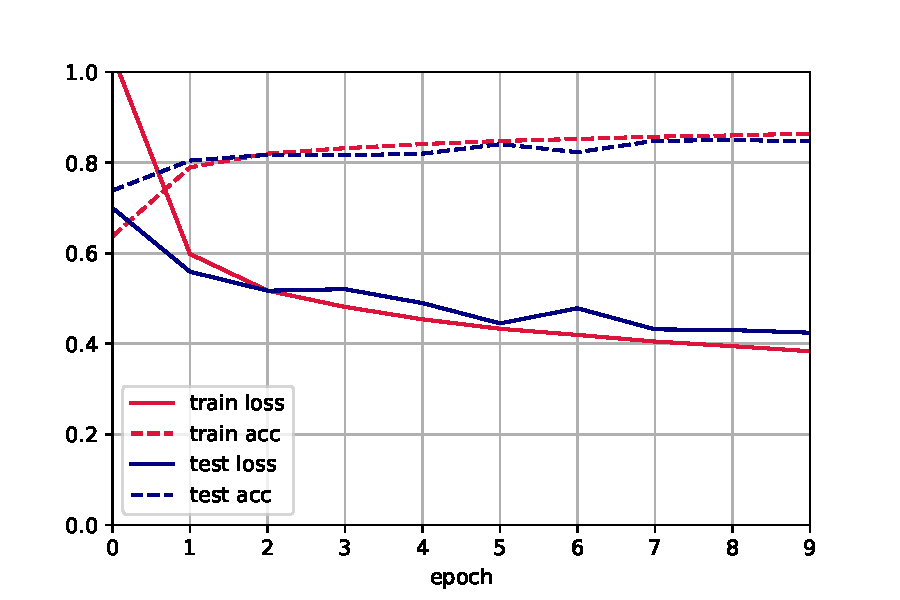
\includegraphics[width=\linewidth]{final_plot}

Code:

\begin{python}
n_inputs = 784
n_hiddens = 256
n_outputs = 10

W1 = torch.randn(size=(n_hiddens, n_inputs), requires_grad=True)
b1 = torch.zeros(n_hiddens, requires_grad=True)
W2 = torch.randn(size=(n_outputs, n_hiddens), requires_grad=True)
b2 = torch.zeros(n_outputs, requires_grad=True)
with torch.no_grad():
    W1 *= 0.01
    W2 *= 0.01



def relu(x):
    return torch.clamp(x, min=0)



def softmax(X):
    Xexp = torch.exp(X)
    return torch.div(Xexp, torch.sum(Xexp, dim=1).unsqueeze(1))



def net(X):
    X = X.flatten(start_dim=1)
    H = relu(X@W1.T + b1)
    return softmax(H@W2.T + b2)



def cross_entropy(y_hat, y):
    return -1. * torch.log(torch.gather(y_hat, 1, y.unsqueeze(1)))



def sgd(params, lr=0.1):
    with torch.no_grad():
        for i in range(len(params)):
            params[i] -= lr * params[i].grad
        for i in range(len(params)):
            params[i].grad.zero_()



def train(net, params, train_iter, loss_func=cross_entropy, updater=sgd):
    for _ in tqdm(range(epochs)):
        for X, y in train_iter:
            y_hat = net(X)
            l = loss_func(y_hat, y).mean()
            l.backward()
            updater(params)

\end{python}


\newpage
%%%%%%%%%%%%%%%%%%%%%%%%%%%%%%%%%%%%%%%%%%%%%
% Name and Calibration
%%%%%%%%%%%%%%%%%%%%%%%%%%%%%%%%%%%%%%%%%%%%%
\subsection*{Name}
Rob Walker

\subsection*{Collaborators and Resources}
Whom did you work with, and did you use any resources beyond cs181-textbook and your notes?
James Kitch, Julian Schmitt, Luke Bailey (OH on Thursday night in Mather), https://pytorch.org/docs/stable/index.html

\subsection*{Calibration}
Approximately how long did this homework take you to complete (in hours)? 25


\end{document}
